\section {Sistema de Clasificación y Lavado de Botellas}
A lo largo de este capítulo se analiza un caso hipotético de uso.
Dicho caso sirve como ejemplo para demostrar las funcionalidades que ofrece el
framework. El mismo consiste en un sistema de clasificación y lavado de
botellas.
A continuación se describen las principales características del mismo:

\begin{itemize}
  \item El ingreso de botellas no es controlado por el sistema.
  \item Las botellas pueden ser depositadas en la máquina en cualquier instante
  de tiempo, de forma asincrónica para el sistema.
  \item La clasificación de las botellas se realiza en un módulo que
  diferencia entre cerveza, gaseosa u otras.
  \item El proceso completo de lavado para una botella de gaseosa consta de los
  siguientes pasos:
	  \begin{itemize} 
	    \item Lavado con agua a presión.
	    \item Secado.
	  \end{itemize}
  \item El proceso completo de lavado para una botella de cerveza consta de los
  siguientes pasos:
	  \begin{itemize} 
	    \item Lavado con agua a presión y detergente.
	    \item Enjuague.
	    \item Secado.
	  \end{itemize}
  \item Si se inserta una botella de otro tipo, la misma es expulsada de la
	máquina sin lavar.
\end{itemize}

\begin{figure}[H]
	\centering
	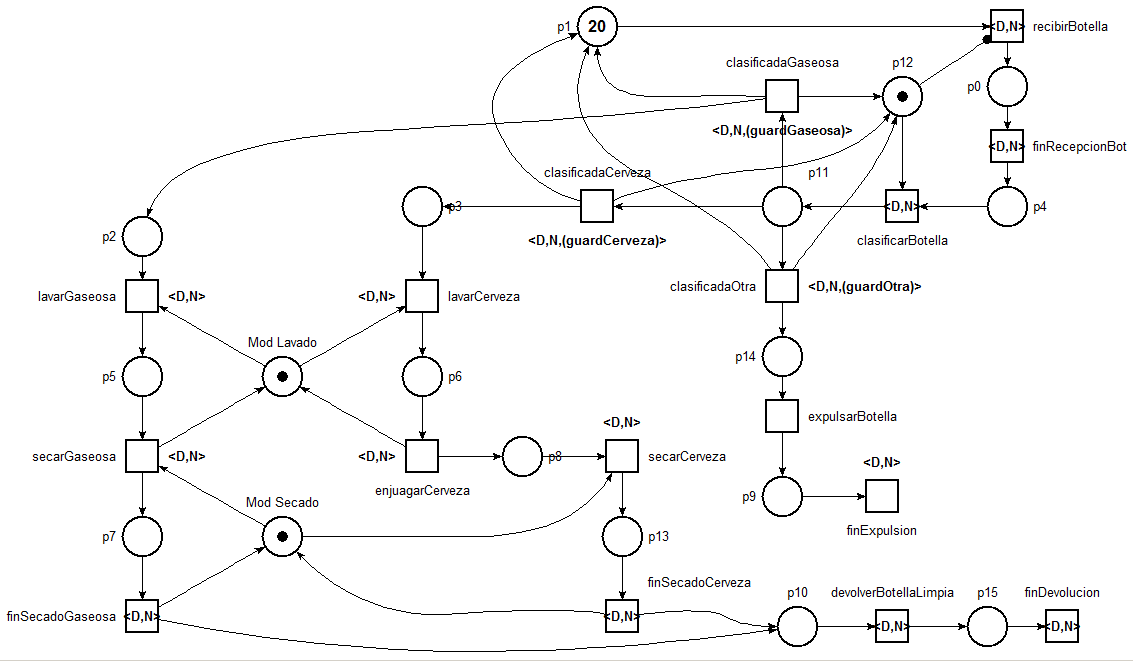
\includegraphics[width=120mm]{petri_lavadora_botellas}
	\caption{Modelo en Red de Petri de la Lógica de un Sistema de Clasificación y
	Lavado de Botellas}
	\label{fig:petri_lavadora_botellas}
\end{figure}

\subsection {Problemas a Resolver}

A continuación se divide la implementación del sistema a partir
de los principales problemas a resolver durante su desarrollo. De esta forma se
comprende facilmente el proceso para crear un sistema utilizando el framework.

\begin{enumerate}
\item \textbf{Determinar los objetos para conformar el sistema:}\\
		Como en cualquier desarrollo orientado a objetos, uno de los pasos principales
		del diseño es la identificación de los objetos que intervienen en el sistema,
		para luego obtener las clases.
		En este caso se identifican los siguientes:
			\begin{itemize}
			  \item Cola de botellas insertadas.
				  \begin{figure}[H]
					\centering
					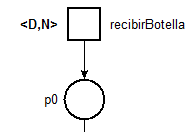
\includegraphics[width=30mm]{ejemplo_Objeto4}
				  \end{figure}
			  \item Módulo de clasificación de botellas.
			  	  \begin{figure}[H]
					\centering
					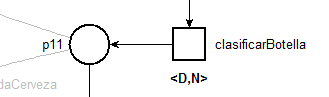
\includegraphics[width=50mm]{ejemplo_Objeto5}
				  \end{figure}
			  \item Módulo de lavado.
			      \begin{figure}[H]
					\centering
					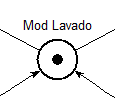
\includegraphics[width=20mm]{ejemplo_Objeto1}
				  \end{figure}
			  \item Módulo de enjuague.
			        \begin{figure}[H]
						\centering
						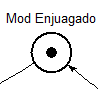
\includegraphics[width=20mm]{ejemplo_Objeto3}
				    \end{figure}
			  \item Módulo de secado.
			        \begin{figure}[H]
						\centering
						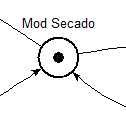
\includegraphics[width=20mm]{ejemplo_Objeto2}
				    \end{figure}
			\end{itemize}

\item \textbf{Determinar las acciones de los objetos del sistema:}\\
			Otro paso principal en el desarrollo orientado a objetos es determinar las
			acciones que pueden realizar los objetos del sistema. Estas acciones serán
			embebidas en los métodos controladores de acciones de las clases
			desarrolladas.

\item \textbf{Determinar la relación entre la Red de Petri, los métodos y las clases:}\\
			La ejecución de un método perteneciente a un objeto está relacionada con el
			disparo de una transición en la Red de Petri. Para eso hay que establecer la
			forma de relacionar dichas transiciones con los objetos y métodos
			correspondientes.
			
			
\end{enumerate}
